\chapter [Deployment and Results]{Deployment and Results}

\epigraph{"Testing leads to failure, and failure leads to understanding"}{Burt Rutan}

In this chapter is presented the experimental setup used to deploy and test the proposed architecture. First is described the data and hardware and software specifications. Then, the two implemented configurations of the system are presented and finally, results are summarized and analysed.

\section{Experimental Setup}

\begin{figure}[ht!]
\centering
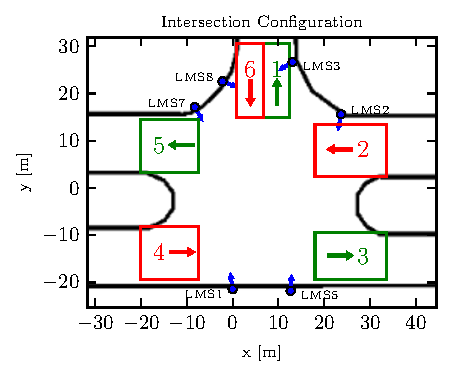
\includegraphics[scale=0.8]{fig/4/intersection-config2.pdf}
\caption{Possi dataset configuration}
\label{possi_img}
\end{figure}

\begin{figure}[ht!]
\centering
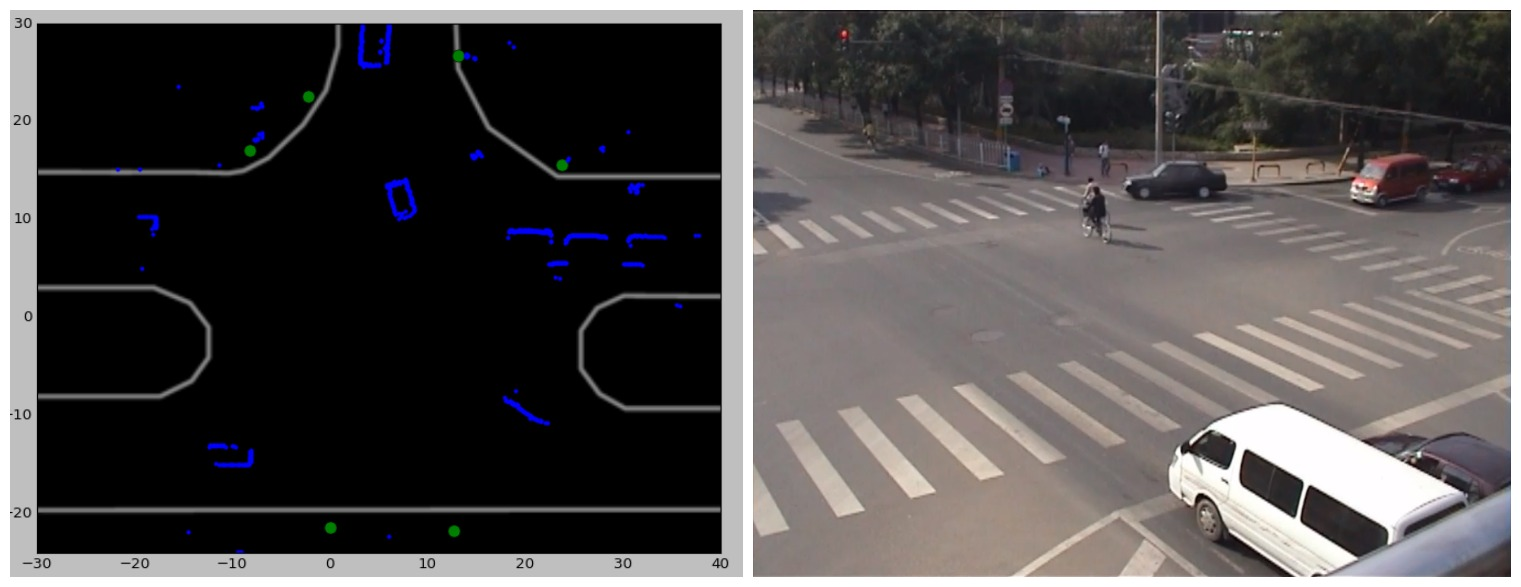
\includegraphics[scale=0.2]{fig/4/sensors_overview.jpeg}
\caption{Overview of sensors data. Left: Laser scanners, Right: Camera.}
\label{possi_sensors}
\end{figure}

%\subsection{Data}
The selected dataset for testing the system is the one from POSSi project (section \ref{possi_ds}). It contains 6 laser-scanners raw readings and a video from a camera located over the intersection. Figure \ref{possi_img} depicts the configuration used by this dataset. In figure \ref{possi_sensors} is shown the data from each type of sensors, laser scanners and camera. The ground truth data used for validation is the vehicle count over 3 of the 5 legs of the intersection, taking into account the time at which a vehicle appears. This groundtruth data was generated manually.

 
%\subsection{Hardware and software specifications}

The platform used for the implementation is a laptop ASUS GL552VW, with 8GB RAM DDR4, a processor Intel Core i7 6700HQ @ 2.60GHz x 8 cores and graphic card Nvidia GeForce GTX 960M. The operating systems running on it is Ubuntu 16.04 LTS. The software was developed using primarily Python3 and C++ as programming languages. Used libraries are MatplotLib, Scikit, Numpy, OpenCV, and darknet for data processing and visualisation. For communication scheme redis was installed along some JSON parsers for formatting.

\section{Test Configurations}
In order to test the proposed architecture, two different configurations have been selected. The first configuration is using just the camera information. The second configuration is based on multiple laser sensors along with the camera.

Each configuration consists of a set of processing blocks (as described in section \ref{proc_blocks}) connected, aiming to take data from  lasers and cameras, to produce an output of higher level. In this case, vehicle counting is the metric used for evaluation.

The following table lists all used blocks and assigns an ID for each one. Those IDs are used in the graph description in its own section. Also, bold nodes and connections indicate multiple instance of the same element.

\begin{table}[ht!]
\footnotesize
\centering
\begin{tabular}{|c | c| c|}
\hline
\textbf{Block ID} & \textbf{Name} \\
\hline
A & laser\_publisher \\
\hline
B & laser\_bg\_remover \\
\hline
C & laser\_pol2cart \\
\hline
D & laser\_cart\_merge \\
\hline
E & points2clusters \\
\hline
F & clusters\_veh\_counter \\
\hline
G & veh\_counter\_merge \\
\hline
H & clusters2occ\_level \\
\hline
I & occ\_level\_merge \\
\hline
J & laser\_pol2cart \\
\hline
K & points2occgrid \\
\hline
L & occgrid\_merge \\
\hline
M & occgrid\_leg\_counter \\
\hline
N & occgrid2occ\_level \\
\hline
O & camera\_publisher \\
\hline
P & camera\_bg\_remover \\
\hline
Q & camera\_blobs \\
\hline
R & camera\_blobs2occgrid \\
\hline
\end{tabular}
\caption{Description of processing blocks used in test configurations}
\label{desc_test_config}
\end{table}


\subsection{Case 1: Single Camera}

\begin{figure}[ht!]
\centering
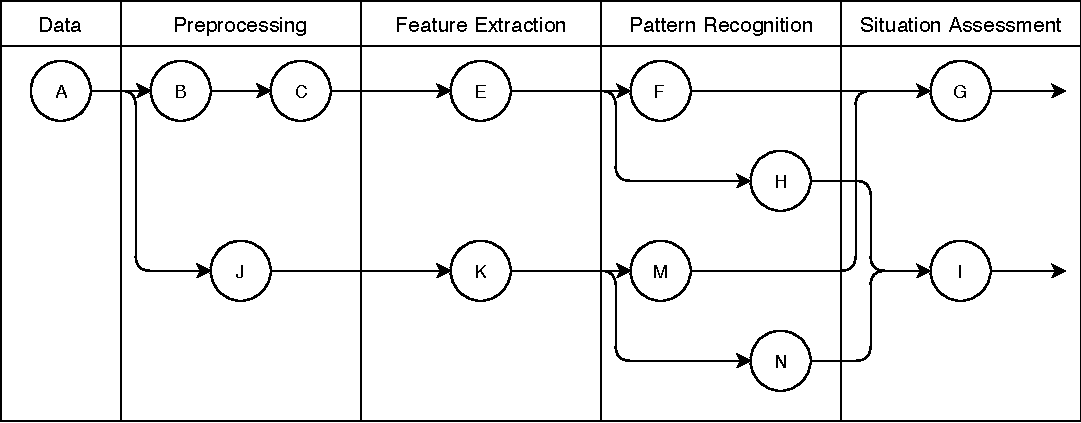
\includegraphics[scale=0.7]{fig/4/test_configuration1.pdf}
\caption{Single laser configuration}
\label{tconf1}
\end{figure}

TODO


\subsection{Case 2: Camera and Multiple Lasers}

\begin{figure}[ht!]
\centering
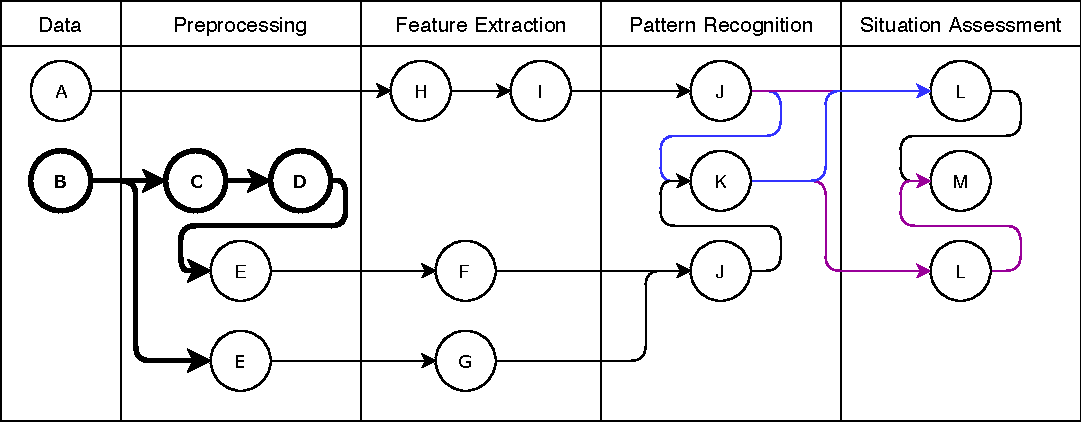
\includegraphics[scale=0.7]{fig/4/test_configuration2.pdf}
\caption{Multiple lasers configuration}
\label{tconf2}
\end{figure}

TODO

%\subsection{Case 3: Multiple Lasers and camera}
%
%\begin{figure}[ht!]
%\centering
%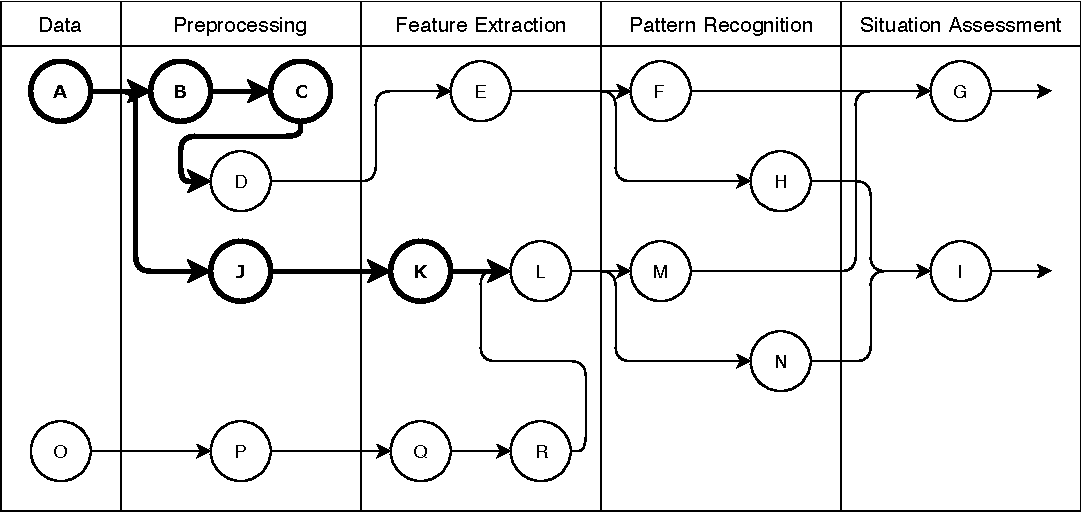
\includegraphics[scale=0.7]{fig/4/test_configuration3.pdf}
%\caption{Multiple lasers and camera configuration}
%\label{tconf3}
%\end{figure}

TODO

\section{Results}

\subsection{Case 1: Single camera}

Detection results in three diferent frames are shown in figure \ref{camera_detection}.

\begin{figure}[ht!]
\centering
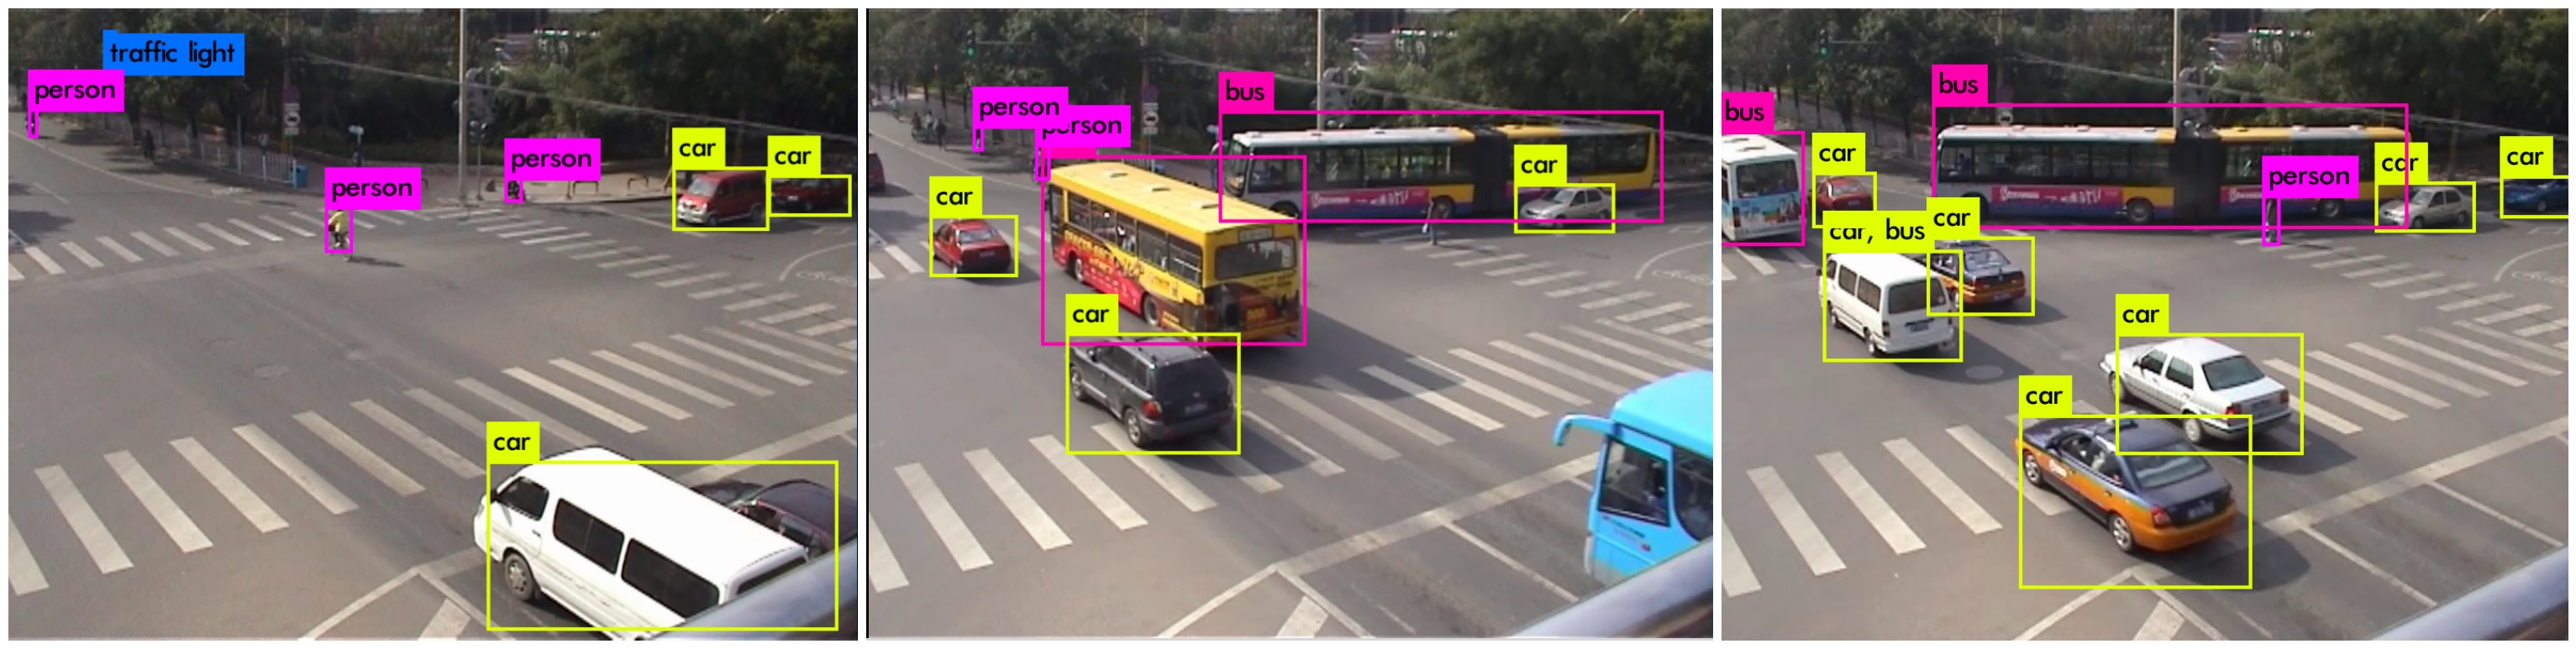
\includegraphics[scale=0.115]{fig/4/camera.jpeg}
\caption{Vehicle detection using camera}
\label{camera_detection}
\end{figure}

\subsection{Case 2: Camera and multple lasers}

Vehicle detection based on laser scanners is shown in figure \ref{laser_detection}.

\begin{figure}[ht!]
\centering
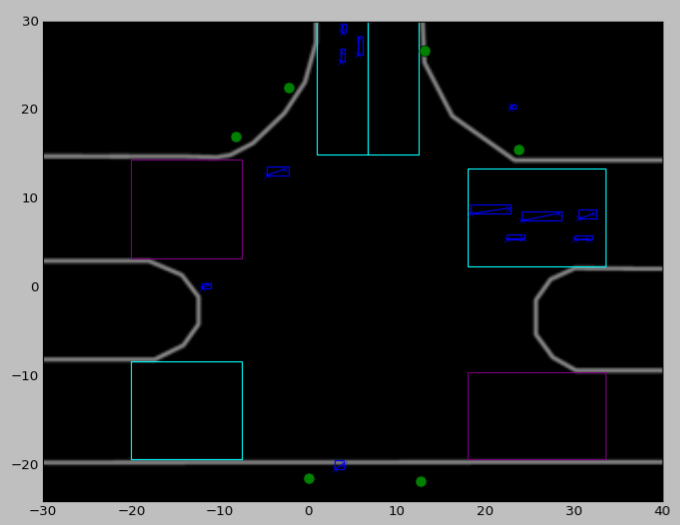
\includegraphics[scale=0.43]{fig/4/laser1.png}
\caption{Vehicle detection using laser scanners}
\label{laser_detection}
\end{figure}

\section{Conclusions}


